\documentclass[a4paper]{article}

\usepackage[english]{babel}
\usepackage[utf8]{inputenc}
\usepackage{amsmath}
\usepackage{graphicx}
\usepackage[colorinlistoftodos]{todonotes}
\usepackage{tikz}
\usetikzlibrary{arrows}
\newcommand{\WP}{\text{WP}}
\newcommand{\CF}{\text{CF}}

\title{Your Paper}

\author{You}

\date{\today}

\begin{document}
\section*{Exercise 1}
\subsection*{a)}
Sequence: \{cloudy, rainy, sunny, sunny\}
$$0.25 \cdot 0.3 \cdot 0.1 \cdot 0.6 = 0.0045$$

\subsection*{b)}
Sequence: \{sunny, snowy, sunny, rainy\}
$$0.25 \cdot 0.0 \cdot 0.0 \cdot 0.1 = 0.0$$

\section*{Exercise 2}
\subsection*{a)}

$\bordermatrix{
  	& 0 	& 1		& 2  	& 3   	& 4   	\cr
0 	& 0 	& p 	& 0 	& 0 	& 1-p	\cr
1 	& 1-p 	& 0 	& p 	& 0 	& 0		\cr
2 	& 0 	& 1-p 	& 0 	& p 	& 0		\cr
3 	& 0 	& 0 	& 1-p 	& 0 	& p		\cr
4 	& p 	& 0 	& 0		& 1-p 	& 0		\cr
}$

\subsection*{b)}
The Markov chain from a) is irreducible. Every state intercommunicates with every other state.

\section*{Exercise 3}
Given transition state matrix:

$$\bordermatrix{
  	& A 	& B		& C  	& D   	\cr
A 	& 1 	& 0 	& 0 	& 0 	\cr
B 	& 0.9 	& 0 	& 0.1 	& 0 	\cr
C 	& 0 	& 0.9 	& 0 	& 0.1 	\cr
D 	& 0 	& 0 	& 0 	& 1 	\cr
}$$
\subsection*{a)}

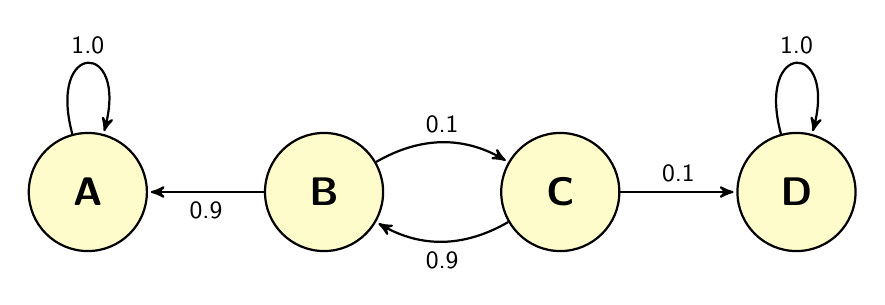
\begin{tikzpicture}[->,>=stealth',shorten >=1pt,auto,node distance=3cm,
  thick,main node/.style={circle,fill=yellow!20,draw,minimum size=1.5cm,font=\sffamily\Large\bfseries}]

  \node[main node] (A) 						{A};
  \node[main node] (B) [right of=A] 	{B};
  \node[main node] (C) [right of=B] 	{C};
  \node[main node] (D) [right of=C] 	{D};

  \path[every node/.style={font=\sffamily\small}]
    (A) edge [loop above] node {1.0} (A)
    (B) edge node {0.9} (A)
        edge [bend left] node {0.1} (C)
    (C) edge [bend left] node {0.9} (B)
        edge node[above] {0.1} (D)
    (D) edge [loop above] node {1.0} (D);
\end{tikzpicture}

\subsection*{b)}
Since we start in state $B$, our initial distribution is given by 
$$\pi^{(0)} = (0,1,0,0).$$

The probability of being in state A after 8 transitions is 
\begin{align*} \pi^{(0)} &\cdot \begin{pmatrix} 
									1 	& 0 	& 0 	& 0 	\\
									0.9 	& 0 	& 0.1 	& 0 \\
									0 	& 0.9 	& 0 	& 0.1 	\\
									0 	& 0 	& 0 	& 1 	
								\end{pmatrix}^8 \\
= (0,1,0,0) &\cdot \begin{pmatrix} 
									1 	& 0 	& 0 	& 0 	\\
									0.988946 	& 0.00006561 	& 0 	& 0.0109883 \\
									0.890051 	& 0 	& 0.00006561 	& 0.0109883 	\\
									0 	& 0 	& 0 	& 1 	
								\end{pmatrix} = (0.988946, 0.00006561, 0, 0.0109883).                                
\end{align*}
Therefore the probability is $0.988946$.

\subsection*{c)}
Since we start in state C, the initial distribution is given by
$$\pi^{(0)} = (0,0,1,0).$$

From the matrix 
$$
\begin{pmatrix} 
1 	& 0 	& 0 	& 0 	\\
0.9 & 0 	& 0.1 	& 0 	\\
0 	& 0.9 	& 0 	& 0.1 	\\
0 	& 0 	& 0 	& 1 	
\end{pmatrix}^6 
= 
\begin{pmatrix} 
1 	& 0 	& 0 	& 0 	\\
0.98829 & 0.000729 	& 0 	& 0.010981 	\\
0.889461 	& 0 	& 0.000729 	& 0.10981 	\\
0 	& 0 	& 0 	& 1 	
\end{pmatrix} 
$$
we can see that the probability of ending in state D after 6 transitions is $0.10.981$

\section*{Exercise 4}
Given sequence of observations: O = \{coffee,coffee,lemonade\}. 

\vspace{5mm}
\noindent Probability matrix:

\begin{tabular}{ l | c | r }
  P & CF & WP \\ \hline
  CF & 0.7 & 0.3 \\
  WP & 0.5 & 0.5 \\
\end{tabular}

\vspace{5mm}
\noindent Emitting probabilities:

\begin{tabular}{ l | c | c | c }
  B & coffee & water & lemonade \\ \hline
  CF & 0.6 & 0.1 & 0.3 \\
  WP & 0.1 & 0.7 & 0.2 \\
\end{tabular}
\subsection*{a) Forward algorithm}
\vspace{5mm}
\begin{tabular}{| c | c | p{3cm} | p{3cm} | p{3cm}|}
  \hline
  state \textbackslash time & $t_0(\text{coffee})$ & $t_1(\text{coffee})$ & $t_2(\text{lemonade})$ & $t_3$\\ \hline
  %
  %
  $\alpha_t(\CF)$ 	& 1 & $1 \cdot 0.7 \cdot 0.6 = 0.42$ 	& $0.42 \cdot 0.7 \cdot 0.6 \newline + 0.18 \cdot 0.5 \cdot 0.1 \newline = 0.1854$ & $0.1854 \cdot 0.7 \cdot 0.3 \newline + 0.0846 \cdot 0.5 \cdot 0.2 \newline = 0.04739$\\ \hline
  %
  $\alpha_t(\WP)$ 	& 0 & $1 \cdot 0.3 \cdot 0.6 = 0.18$	& $0.42 \cdot 0.3 \cdot 0.6 \newline + 0.18 \cdot 0.5 \cdot 0.1 \newline = 0.0846$ & $0.1854 \cdot 0.3 \cdot 0.3 + 0.0846 \cdot 0.5 \cdot 0.2 \newline = 0.02515$ \\ \hline
  %
  P[cof,cof,lem] & 1 & 0.6	& 0.27 & 0.07254 \\ \hline
\end{tabular}

\subsection*{b) Backward algorithm}
\begin{tabular}{| p{3cm} | p{3cm} | p{3cm} | p{3cm} | c|}
  \hline
  state \textbackslash time & $t_0(\text{coffee})$ & $t_1(\text{coffee})$ & $t_2(\text{lemonade})$ & $t_3$\\ \hline
  %
  %
  $\alpha_t(\CF)$ 	& $0.162 \cdot 0.7 \cdot 0.6 \newline + 0.025 \cdot 0.3 \cdot 0.6 \newline = 0.07254 $ 	& $0.3 \cdot 0.7 \cdot 0.6 \newline + 0.2 \cdot 0.3 \cdot 0.6 \newline = 0.162$ 	& $1.0 \cdot 0.7 \cdot 0.3 \newline + 1.0 \cdot 0.3 \cdot 0.3 \newline = 0.3$ 	& $1.0$		\\ \hline
  %f
  $\alpha_t(\WP)$ 	& $0.162 \cdot 0.5 \cdot 0.1 \newline + 0.025 \cdot 0.5 \cdot 0.1 \newline = 0.00935$ 	& $0.3 \cdot 0.5 \cdot 0.1 \newline + 0.2 \cdot 0.5 \cdot 0.1 \newline = 0.025$ 	& $1.0 \cdot 0.5 \cdot 0.2 \newline + 1.0 \cdot 0.5 \cdot 0.2 \newline = 0.2$ 		& $1.0$ 	\\ \hline
  %
  P[cof,cof,lem] & $0.07254$ &	&  &  \\ \hline
\end{tabular}

\subsection*{c)}

\begin{tabular}{| c | c | c | p{4cm} | p{4cm}|}
  \hline
  state \textbackslash time & $t_0(\text{coffee})$ & $t_1(\text{coffee})$ & $t_2(\text{lemonade})$ & $t_3$\\ \hline
  %
  %
  $\delta_t(\CF)$ 	& 1 & $0.42$ 	& $Max[\CF: 0.42 \cdot 0.7 \cdot 0.6 = 0.1764; \WP: 0.18 \cdot 0.5 \cdot 0.1 = 0.009] = 0.1764$ & $Max[\CF: 0.1764 \cdot 0.7 \cdot 0.3 = 0.03704; \WP: 0.0756 \cdot 0.5 \cdot 0.2 = 0.00756] = 0.03704$ \\ \hline
  %
  $\delta_t(\WP)$ 	& 0 & $0.18$	& $Max[\CF: 0.42 \cdot 0.3 \cdot 0.6 = 0.0756; \WP: 0.18 \cdot 0.5 \cdot 0.1 = 0.009] = 0.0756$ & $Max[\CF: 0.1764 \cdot 0.3 \cdot 0.3 = 0.01588; \WP: 0.0756 \cdot 0.5 \cdot 0.2 = 0.00756] = 0.01588$ \\ \hline
  %
  %
  $\psi_t(\CF)$&  & \CF	& \CF & \CF \\ \hline
  %
  $\psi_t(\WP)$&  & \CF	& \CF & \CF \\ \hline
  %
  $x_t$ & \CF & \CF & \CF &  \\ \hline
\end{tabular}

\vspace{5mm}
\noindent For the given observations O = \{coffee,coffee,lemonade\}, the most probable sequence of states is therefore \{\CF, \CF, \CF\}.


\end{document}